\documentclass[11pt]{article}
\usepackage[toc,page]{appendix}
\usepackage{amsmath, amssymb}
\usepackage[utf8]{inputenc}
\usepackage[T1]{fontenc}
\usepackage[style=apa,backend=biber]{biblatex}
%\usepackage{biblatex}
\addbibresource{references.bib}
\usepackage{graphicx}
\usepackage{tikz}
\usetikzlibrary{automata,positioning,shapes.geometric, arrows.meta, fit, backgrounds, calc, chains}
\graphicspath{./images/Easy_Pictures/SMR_MULT_Repackaging}%\usepackage{kpfonts}
\usepackage{float}
\usepackage[margin=1in]{geometry}
\usepackage{cancel}
\usepackage{epsfig}
\usepackage{tikz-3dplot}
\usepackage{darkmode}
\usepackage{dirtytalk}
\usepackage{longtable,booktabs,array}
\usepackage{calc} % for calculating minipage widths
\usepackage[utf8]{inputenc}
\usepackage[T1]{fontenc}
\usepackage{xcolor}
\usepackage{listings}


\usepackage{etoolbox}
\usepackage{hyperref}
\hypersetup{
    colorlinks=true,
    linkcolor=blue,
    filecolor=magenta,      
    urlcolor=cyan,
    pdftitle={Hermeneutic Calculator},
    citecolor=blue,
    }


\urlstyle{same}

\lstdefinestyle{htmlStyle}{
    language=HTML,
    basicstyle=\ttfamily\small,
    keywordstyle=\color{blue}\bfseries,
    commentstyle=\color{gray}\itshape,
    stringstyle=\color{red},
    breaklines=true,
    frame=single,
    numbers=left,
    numberstyle=\tiny\color{gray},
    columns=fullflexible,
}
\lstdefinelanguage{HTML}{
  keywords={<!DOCTYPE, html, head, title, body, h1, h2, h3, p, div, span, a, img, ul, li, table, tr, td, th, style, link, script},
  sensitive=true,
  comment=[l]{//},
  morecomment=[s]{/*}{*/},
  morestring=[b]',
  morestring=[b]"
}
\lstset{style=htmlstyle, language=html}
% Updated to explicitly pass the language option
%\lstinputlisting[style=htmlstyle, language=html]{./html/example.html}
%\usepackage{tocloft}

% Optional: define some custom colors
\definecolor{sliceRed}{RGB}{225,224,91} % matching "varyellow" from your code
\definecolor{linkYellow}{RGB}{255,215,0}  % a golden yellow
\tdplotsetmaincoords{70}{110}

\title{Strategic Multiplicative Reasoning: Conversion to Bases and Ones (CBO)}
\author{Compiled by: Theodore M. Savich}


\begin{document}
\maketitle
\subsection*{Transcript}
Strategy descriptions and examples adapted from \textcite{HackenbergCourseNotes}. 


\begin{itemize}
    \item \textbf{Teacher:} You have 7 mini cans of soda. Each can has 9 ounces of soda in it. How many
    ounces of soda do you have total?
    \item \textbf{George:}  Well, you could take one of the 9 ounces and put an extra ounce into all other
    cans. That would give you 6 tens with 3 ounces leftover. So, 63.
    \item \textbf{Teacher:} Great!
\end{itemize}


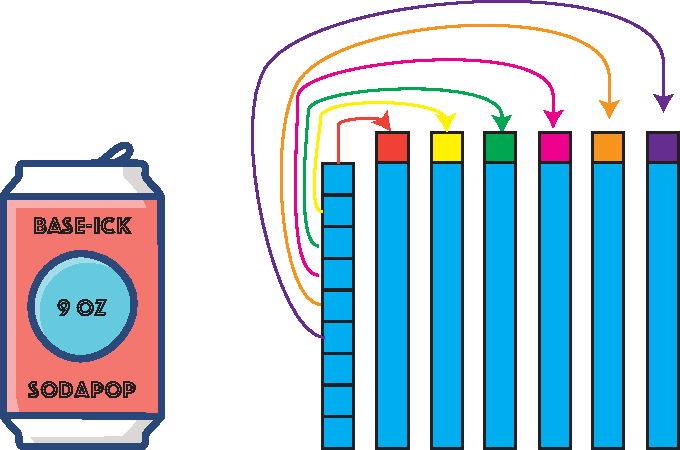
\includegraphics[width=.8\textwidth]{images/Easy_Pictures/SMR_CBO/PDF/SMR_CBO_Soda.pdf}

\begin{align*}
    \text{Seven} \times 9 &= \text{Six} \times 9 + 9  \\
    &=  \text{Six} \times 9 + 6 + 3 \\
    &= \text{Six}\times (9+1) +3  \\
    &= \text{Six}\times 10 + 3 \\
    &=63
    \end{align*}

Begin with groups of a known size. The objective is to form groups that equal the base size. To achieve this, break one group apart and redistribute its individual units to other groups until they form complete bases; repeat with additional groups if necessary. Typically, some units will remain ungrouped. The total count is then the sum of the complete bases and any leftover units.
\subsection*{Conversion to Bases and Ones (CBO)}

\subsubsection*{Description of Strategy:}
\begin{itemize}
    \item \textbf{Objective:} Rearrange the items from groups to make complete base units by combining ones from different groups.
    \item \textbf{Method:} Break apart groups and redistribute ones to form full base units (e.g., tens).
\end{itemize}

\subsubsection*{Automaton Type:}
\textbf{Pushdown Automaton (PDA)}: The stack is used to represent the redistribution of ones in order to form complete base units.

\subsubsection*{Formal Description of the Automaton}

We define the PDA as the 7-tuple
\[
M = (Q,\, \Sigma,\, \Gamma,\, \delta,\, q_{0/accept},\, Z_0,\, F)
\]
where:
\begin{itemize}
    \item \(Q = \{q_{0/accept},\, q_{\text{collect}},\, q_{\text{form}}\}\) is the set of states. Here, \(q_{0/accept}\) serves as both the start and accept state.
    \item \(\Sigma\) is the input alphabet (encoding the group information, e.g., number of groups and ones per group).
    \item \(\Gamma = \{Z_0\} \cup \{1\}\) is the stack alphabet, where \(Z_0\) is the initial stack symbol and the symbol \(1\) represents a single one.
    \item \(q_{0/accept}\) is the start state, which is also the accept state.
    \item \(F = \{q_{0/accept}\}\) is the set of accepting states.
\end{itemize}

The transition function \(\delta\) is defined by:
\begin{enumerate}
    \item \(\delta(q_{0/accept},\, \text{``init''},\, Z_0) = \{(q_{\text{collect}},\, Z_0)\}\) \\
          (Initialize the process to collect ones from the groups.)
    \item In state \(q_{\text{collect}}\):  
          \(\delta(q_{\text{collect}},\, \varepsilon,\, x) = \{(q_{\text{collect}},\, 1x)\}\) for any \(x \in \Gamma\) \\
          (For each group, push the ones (e.g., \(S\) ones) onto the stack.)  
          \\
          Additionally, when all groups have been processed (i.e. a designated input symbol signals that the count of groups equals \(N\)), we have:  
          \(\delta(q_{\text{collect}},\, \varepsilon,\, Z_0) = \{(q_{\text{form}},\, Z_0)\}\).
    \item In state \(q_{\text{form}}\):  
          \(\delta(q_{\text{form}},\, \varepsilon,\, 1) = \{(q_{\text{form}},\, \varepsilon)\}\) (simulate popping a one) repeated until fewer than \(BSize\) symbols remain on the stack.  
          When fewer than \(BSize\) ones remain (i.e., a full base unit cannot be formed),  
          \(\delta(q_{\text{form}},\, \varepsilon,\, Z_0) = \{(q_{0/accept},\, Z_0)\}\) \\
          (Output the final result, which is implicitly represented by the distribution of ones on the stack.)
\end{enumerate}

\subsubsection*{Automaton Diagram for Conversion to Bases and Ones}

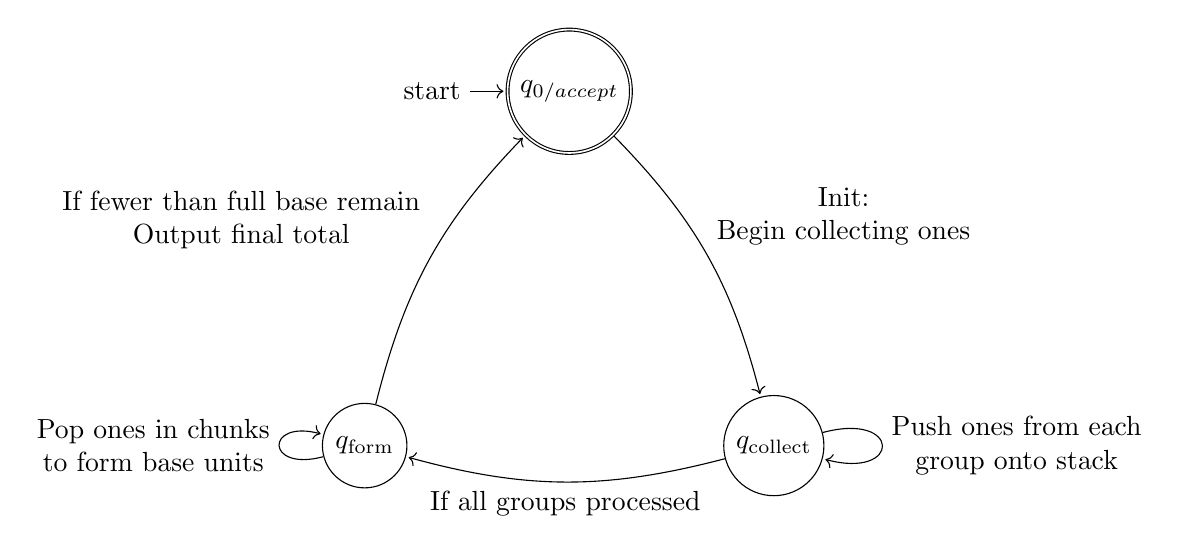
\begin{tikzpicture}[
    shorten >=1pt,
    auto,
    node distance=3cm,
    every state/.style={minimum size=1cm}
]
    % Arrange three states on a circle:
    \node[state, initial, accepting] (q0) at (90:3cm) {$q_{0/accept}$};
    \node[state] (q1) at (330:3cm) {$q_{\text{collect}}$};
    \node[state] (q2) at (210:3cm) {$q_{\text{form}}$};

    \path[->]
        (q0) edge[bend left=15] node[above right, align=center] {Init:\\Begin collecting ones} (q1)
        (q1) edge[loop right] node[right, align=center] {Push ones from each\\group onto stack} (q1)
        (q1) edge[bend left=15] node[below, align=center] {If all groups processed} (q2)
        (q2) edge[loop left, looseness=7] node[left, align=center] {Pop ones in chunks\\to form base units} (q2)
        (q2) edge[bend left=15] node[above left, align=center] {If fewer than full base remain\\Output final total} (q0);
\end{tikzpicture}


\clearpage

\subsubsection*{HTML Implementation}
\lstinputlisting[style=htmlStyle, language=html]{./new_html/SMR_Multiplication_CBO.html}

\printbibliography
\end{document}